\section{Busca de elementos regulatórios}

   \frame{\justifying
    \frametitle{Busca por padrões}
    	\begin{itemize}
    		\item A busca por elementos regulatórios remete a busca por padrões em uma \textit{string}.
    		\item Dado um padrão de DNA, encontrar sequências candidatas é simples, mas diferenciar sítios reais dos não reais é difícil.
    		\begin{itemize}
				\item Um fator de transcrição específico utilizado na expressão de um determinado gene, pode não ser o mesmo para a expressão de outro gene. Entretanto um único também TF pode regular múltiplos genes.
% Experimentos com microarray mostraram que, quando um gene X não é expresso, outros 20 não são expressos, uma vez que o gene X codifica proteinas reguladoras TFs, o 20 genes não expressos são regulados pelos TFs do gene X. 		 
				\item Essa especificidade torna os elementos regulatórios em sequências que não são consenso.

%Um fator de transcrição específico utilizado na expressão de um determinado gene, pode não ser o mesmo para a expressão de outro gene. Por exemplo o conjunto de fatores de transcrição de uma célula óssea no organismo humano, pode ter fatores diferentes do conjunto de TFs de uma célula do figado, uma vez que essas diferentes células podem precisar de diferentes proteínas. Essa especificidade torna os elementos regulatórios em sequências que não são consenso, em consequência os elementos regulatórios não seguem um padrão.	
	    	
	    		\item Pelo fato que muitos elementos regulatórios são usualmente degenerados, sofrem mutações, deleção ou inserção.	
    		\end{itemize}
    	\end{itemize}
	}
	
   \frame{\justifying
    \frametitle{Um exemplo da degeneração}
		\begin{figure}[htb!]
		    \centering
		    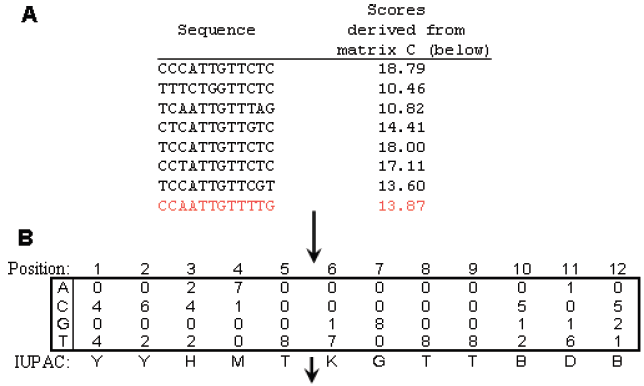
\includegraphics[scale=0.5]{./imagens/ET_caso_element1.png}
		    \caption{Oito conhecidos elementos regulatórios da \textit{Saccharomyces cerevisiae}, a pontuação esta de acordo com a PWM em C}
		    \label{fig:ET_caso_element1}
		\end{figure}		
	}	

   \frame{\justifying
    \frametitle{Um exemplo da degeneração}
		\begin{figure}[htb!]
		    \centering
		    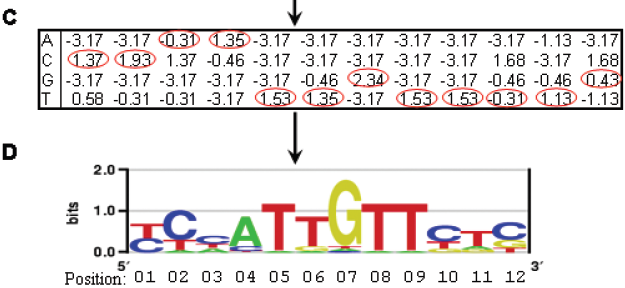
\includegraphics[scale=0.5]{./imagens/ET_caso_element2.png}
		    \caption{Matriz de peso das sequências alinhadas e a representação logo da sequência}
		    \label{fig:ET_caso_element2}
		\end{figure}		
	}	

   \frame{ \justifying
    \frametitle{Um exemplo da degeneração}
		Os valores da matriz de peso mostrada em C são obtidos calculando:
		$ \log_{2}(f_{i,j}/P_{i})$, onde $f_{i,j}$ é a frequência da base $i$ na posição $j$. Este valor pode ser obtido dividindo o valor da célula da matriz pelo numero de sítios na posição (p.e $f_{C,1} = f_{T,1} = 4/8 = 0.5$). E $P_{i}$ é a probabilidade de encontrar uma base na posição $i$, que é $P_{A} = P_{T} = 0.32$, e $P_{C} = P_{G} = 0.18$ (valor correspondente ao genoma do \textit{S.cerevisiae}).
	}	

	
%A busca por padrão pode ser descrita como, dado um conjunto de sequências de DNA e um tamanho L, o objetivo é identificar os padrões  mais significantes de tamanhos L. Como solução podemos gerar todos os possíveis padrões na sequência, então buscar o numero de ocorrência de cada padrão, reportando os que tiverem a maior frequência, como sendo os mais significativos. Este tipo de técnica garante bons resultados, até mesmo em padrões degenerados. Porém a procura por padrões com tamanhos grandes em um espaço de 4^L, têm um grande custo computacional, fazendo que se torne inviavel para buscas com L > 10. Para contornar este problema recorre-se ao uso de dados pré-processados, para diminuir o espaço e a busca se tornar menos custosa. Ou combinar a sobreposição de pequenos padrões encontrados para encontrar padrões maiores e mais complexos. Também, pode-se usar arvores sufixas que diminuem a complexidade e aumenta o tamanho de L. Estes tipos de abordagens também são conhecidas como abordagens de busca baseada em palavras.

%Nos metodos dirigidos pelas sequências o objetivo é encontrar a localização dos motifs e a PWM representativa usando apenas os dados da sequência, como a informação da localização dos motifs não é conhecida, está informação tem que ser aprendida. Para isto utiliza-se algoritmos de aprendizagem de maquina. Varios algoritmos foram propostos utilizando esta abordagem, como algoritmos gulosos, expectation-maximization (EM), Gibbs samplis entre outros.

%Outras abordagens  que vêm se destacando são: o de comparação entre os genomas para a busca dos elementos reguçatórios e da busca de modulos de elementos regualtórios.
	
   \frame{\justifying
    \frametitle{Busca de elementos regulatórios}
		\begin{itemize}
			   \item Para contornar esses problemas foram desenvolvidos vários algoritmos de busca de elementos regulatórios. Eles são classificados em três grupos:
				   \begin{enumerate}
						\item busca de em genes co-regulados
						\item busca em genes ortólogos 		   
						\item busca simultânea em genes ortólogos e co-regulados.
				   \end{enumerate}
		\end{itemize}
}

   \frame{\justifying
    \frametitle{Busca em genes co-regulados}
    	\begin{itemize}
			\item Genes que são regulados pelos mesmos conjuntos de fatores de transcrição.
    	\end{itemize}
    }

   \frame{\justifying
    \frametitle{Busca em genes co-regulados}
		\begin{figure}[htb!]
		    \centering
		    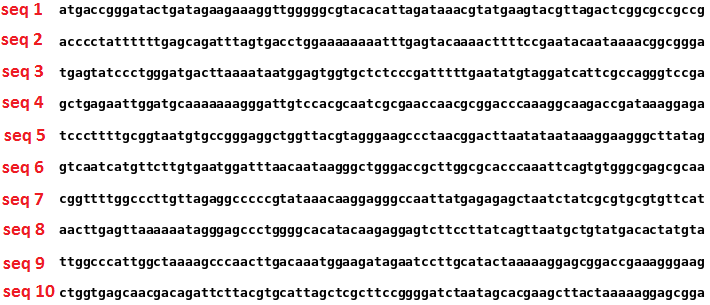
\includegraphics[scale=0.5]{./imagens/exe_element.png}
		    \caption{Diferentes sequências promotoras de uma mesma espécie}
		    \label{fig:exe_element}
		\end{figure}		
	}

   \frame{\justifying
    \frametitle{Busca em genes co-regulados}
		\begin{figure}[htb!]
		    \centering
		    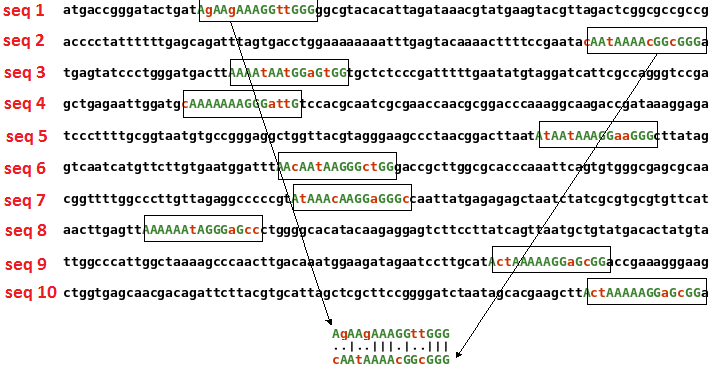
\includegraphics[scale=0.5]{./imagens/exe_element2.png}
		    \caption{Encontrado um padrão nas sequências}
		    \label{fig:exe_element2}
		\end{figure}		
	}


   \frame{ \justifying
    \frametitle{Oligo-Analysis}
    	Um dos métodos propostos para a identificação dos elementos regulatórios em genes co-regulados é o de \cite{Helden1998}. Os autores projetaram um algoritmo que detecta oligonucleotídios (um fragmento curto de DNA) sobre-representados na região promotora dentro de um grupo de genes co-regulados. O programa conta todas as ocorrências dos oligonucleotídios dentro do conjunto de sequências e estima a significância estatística.    	
	}
%	Como uma solução podemos gerar todos os possíveis padrões na sequência, então buscar o numero de ocorrência de cada padrão, reportando os que tiverem a maior frequência, como sendo os mais significativos.

   \frame{ \justifying
    \frametitle{Oligo-Analysis}
		Primeiramente foram calculadas as frequências esperadas $F_{e}\lbrace b \rbrace$ para cada oligonucleotídio $(b)$ de tamanhos de um a nove. Então determinada a ocorrência esperada para cada oligonucleotídio no conjunto de sequências promotoras com a formula $E(occ\lbrace b \rbrace) = F_{e}\{ b \}*T$ onde $T = 2xSx(L - w + 1)$, onde $w$ é a tamanho do oligonucleotídio; $S$ é o numero de sequências no conjunto; $L$ é o tamanho das sequências. O fator 2 é devido a soma de ocorrências é feita em ambos os filamentos de DNA.
	}
   \frame{ \justifying
    \frametitle{Oligo-Analysis}
		A significancia estatística é encontrada através da formula $P(ooc \lbrace b \rbrace = n) = \frac{T!}{(T -n)! x n!} x (F_{e}\{ b \})^n x (1 - F_{e}\{ b \})^(T -n) $. 
	}		
	\frame{ \justifying
    \frametitle{Oligo-Analysis}
	Depois que são encontrados os oligonucleotídios que são sobre-representados (que seguem um padrão) que têm grandes possibilidades de aparecerem em sequências promotoras, então são determinados nas sequências promotoras as posições que batem com os oligonucleotídios encontrados.
	% Probabilidade de encontra n ocorrências do oligonucleotifio b no conjunto de sequências, o com maior probabilidade é escolhido.
	}	
	\frame{ \justifying
    \frametitle{Oligo-Analysis}
	Este tipo de técnica garante bons resultados, até mesmo em padrões degenerados. Porém a procura por padrões com tamanhos grandes em um espaço de $4^L$, onde $L$ é o tamanho da sequência,tem um grande custo computacional, fazendo que se torne inviável para buscas com $L > 10$.	
	}

   \frame{\justifying
    \frametitle{Busca em genes ortólogos}
    	\begin{itemize}
			\item São genes \textit{homólogos} que foram separadas por um evento especial, fazendo que diferentes espécies tenham os mesmos genes.
    	\end{itemize}
%são genes/seqüências que derivaram de ancestrais comuns e conseqüentemente elas são conservadas e apresentam grande similaridade, por exemplo genes homólogos podem ser encontrados em dois diferentes organismos mas que derivaram do mesmo ancestral, por isso possuem o mesmo gene que é homologo entre esses dois organismos.     	
    }

   \frame{\justifying
    \frametitle{Busca em genes ortólogos}
		\begin{figure}[htb!]
		    \centering
		    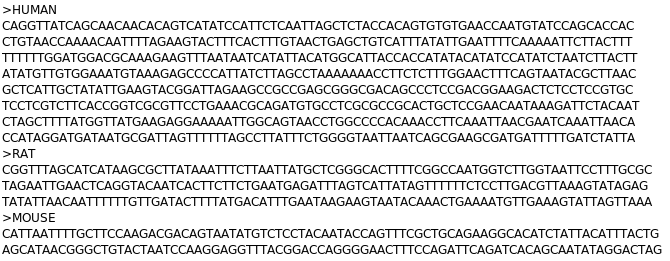
\includegraphics[scale=0.5]{./imagens/exe_seq.png}
		    \caption{Sequências de várias espécies}
		    \label{fig:exe_seq}
		\end{figure}		
	}
	
   \frame{\justifying
    \frametitle{Busca em genes ortólogos}
		\begin{figure}[htb!]
		    \centering
		    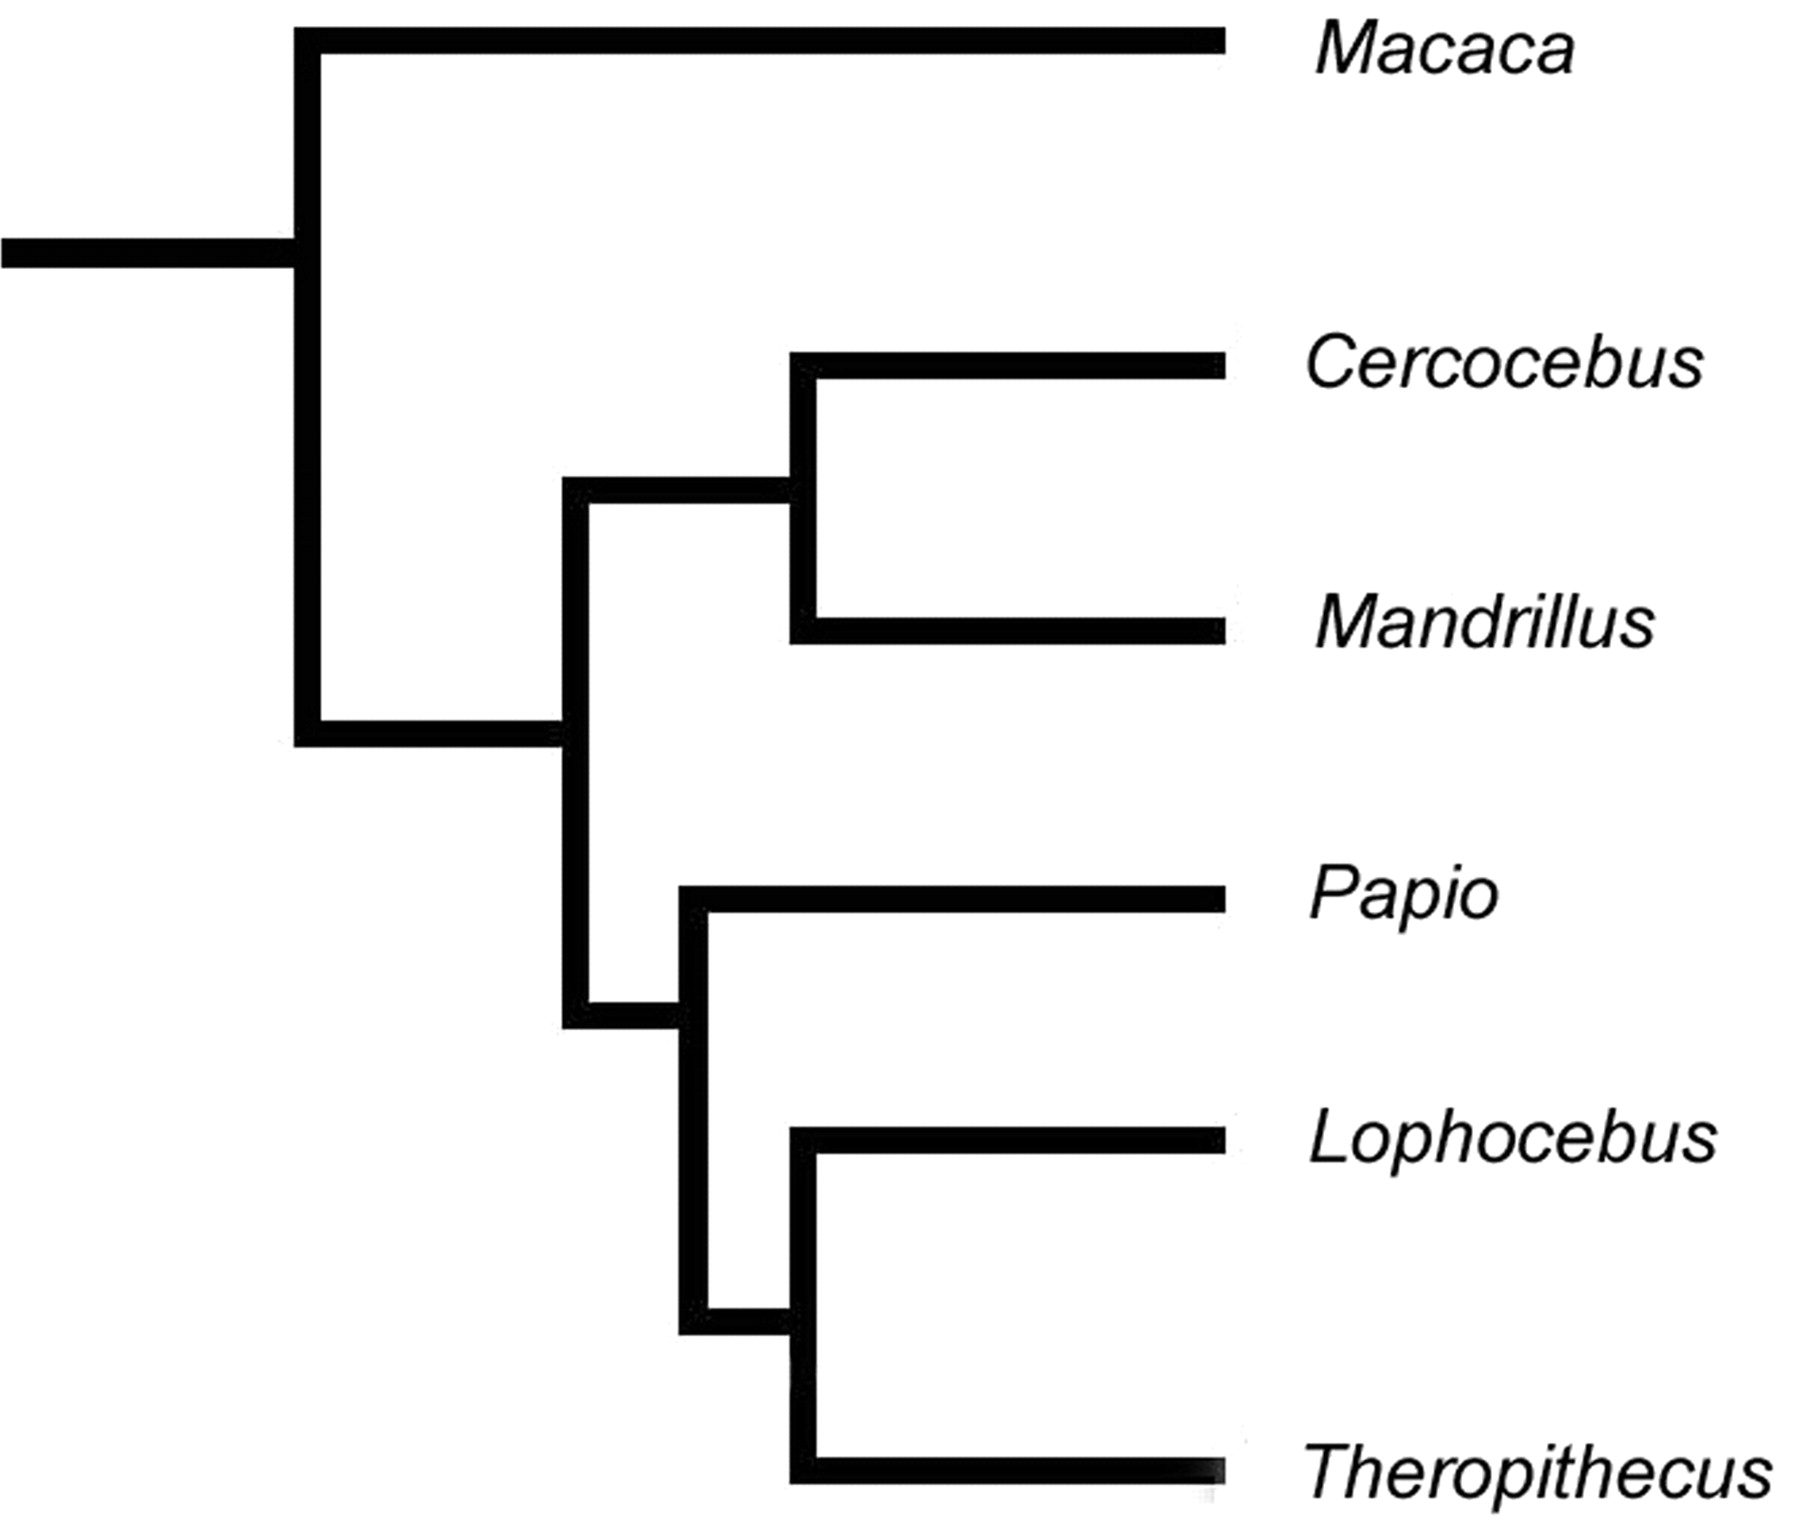
\includegraphics[scale=0.1]{./imagens/phy_tree.jpg}
		    \caption{Árvore filogenética}
		    \label{fig:phy_tree}
		\end{figure}		    	
	}

   \frame{\justifying
    \frametitle{FootPrinter}
    	\begin{itemize}
    		\item Este algoritmo \cite{Blanchette2002} tem como entrada uma a árvore filogenética e as sequências $s$ promotoras de várias espécies e o tamanho do elemento regulatório.
    		\item É calculado a menor pontuação de parcimônia da sub-árvore $d_{v}^* = \sum_{w \in C(v)} min_{t' \in \sum^{k}}(d_{w}^*(t')+d(t',t)$ até a raiz.
    		\item Então é gerado sequências randômicas $r$ que simulam a evolução das sequências $s$ mas sem pressão natural.
    		\item Calula-se a divergência entre $s$ e $r$.
    		\item $s$ e $r$ têm a mesma frequência de nucleotídeos.    		
    	\end{itemize}
	}
	